\chapter{Olivia} \label{chapter:Olivia}

\section{Overview}
Olivia is the microservice responsible for extracting attributes from an image, named after Olivia Wilson as the technology used in the service utilises her work done during her Masters project. Note that all references to ‘Olivia’ are referring to this microservice. Taking Olivia from a black box perspective, it take a 256 by 256 pixel image and returns a corresponding attribute vector (of 1024 elements) that `describes’ the image. 


\begin{figure}[H]
    \centering
    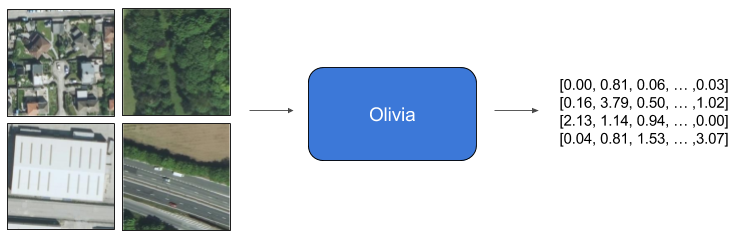
\includegraphics[width=\textwidth]{figs/7/olivia-goal}
    \caption{Visual Description of Olivia}
    \label{fig:basic_olivia}
\end{figure}


Attribute extraction for images is a complex task, and there are many questions that need to be asked. How attributes should be extracted from images? How many attributes should be extracted? What attributes are necessary to distinguish each image uniquely? How do you determine when a feature starts and finishes? Wilson’s work answers many of these questions, but also introduces others, some of which are solved in this project. 

This microservice was designed to act as both a standalone service and module within a system (like this project). It has its own HTTP endpoints, persistence and control sequences, all of which allow it to be used independently from the other services in the system.


\section{Background Research}

\subsection{Terrapattern}

Terrapattern (discussed in section \ref{section:existing:terrapattern}) evidently has a fantastic attribute extraction module. It has an impressive ability for recognising edge cases, and despite often finding differences between images that a human would believe to be identical, this only provides further evidence that it can extract a vast number of attributes to identify such subtle differences. 

On further inspection of the public source code (\url{https://github.com/CreativeInquiry/terrapattern}), it seems rather evident that there is a private side to the repository that the website is using. The code available uses six different languages and the submodules contained are written in an additional three languages. Despite being open source, the codebase seems so obfusticated that it is unusable. 

\subsection{Wilson’s Work}

Wilson’s paper, entitled ``Incorporating scale into convolutional neural networks for use on aerial image interpretation” and commissioned by OS, looks into extending a deep neural network to increase image classification of map tiles. This new neural network (now 17 neural network nodes) accepts a 256 by 256 pixel image and classifies the centre pixel based on the surrounding 192 by 192 pixels (as can be seen in figure \ref{fig:olivia_range}). As this project and ours are commissioned by OS, the code is available with assistance from Wilson and others.

\begin{figure}[H]
    \centering
    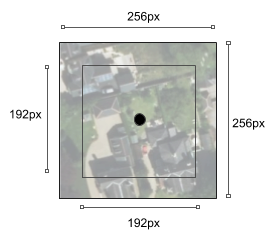
\includegraphics{figs/7/tile_range}
    \caption{Olivia Classification Visualisation}
    \label{fig:olivia_range}
\end{figure}


\section{Design}

Olivia has a single responsibility: to extract attributes when provided with map tile images. While this can be a slow process, it has been optimized in order to fulfill this responsibility without significantly impacting the user experience. The main case flow is quite simple: when given an image, check if the image has been seen before. If so, return the vector previously computed. Otherwise, convert the image to an attribute vector, remember it and return the vector. 

\begin{figure}[H]
    \centering
    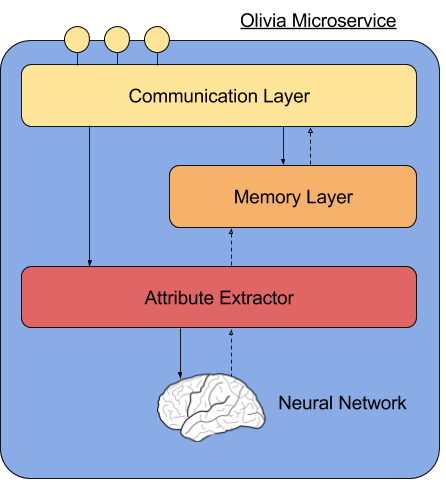
\includegraphics[width=8cm]{figs/7/olivia_design}
    \caption{Olivia Microservice Design}
    \label{fig:olivia_design}
\end{figure}

A number of decisions had to be made when considering the design and implementation of this mircoservice:

\subsection{Wilson’s Code or Terrapattern}

Having seen Terrapattern’s website, it looked like a prototype that could have been extended to match the requirements of the project. However as mentioned in section \ref{section:existing:terrapattern}, the code was unusable and included using experimental languages. 

Wilson’s code, in comparison, could be deconstructed to use the trained deep neural network (DNN) for attribute extraction. Originally, the network produced four outputs, corresponding to the probability of the image belonging to four major themes. The number of nodes in neural networks diverge as they reach the centre of the network and then converge towards the output layer. To increase the output of Wilson’s DNN, we removed the last four layers resulting in an output of 1024 non-negative doubles that are the decomposition of the image (shown in figure \ref{fig:NN_decomp}). Due to the issues with Terrapattern, the use of Wilson’s code was chosen. 

\begin{figure}[H]
    \centering
    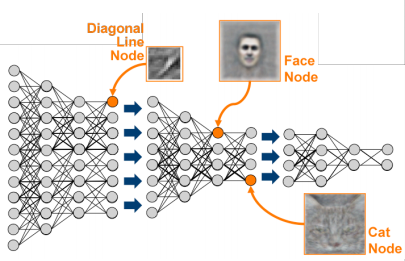
\includegraphics[width=12cm]{figs/7/NN_decomp}
    \caption{A visualization of a NN classifying images \citep{murnane_2016}}
    \label{fig:NN_decomp}
\end{figure}
	
\subsection{GPU or CPU}

The DNN produced by Wilson runs on a nervana module that works on tensor flow. This supports uses the processor or graphics card to compute the output of the DNN. Comparing the two, the processor is easy to setup and easier to maintain. Using the graphics card is complex and somewhat unreliable. Under experiments, the CPU processed one image every 30 seconds, whereas the GPU completed 128 images every tenth of a second. The speed of CPU prevented it from being a viable solution hence GPU processing was chosen. 

\subsection{Wilson Ignores Border Issue} \label{section:nsew}

As can be seen in \ref{fig:olivia_range} (page \pageref{fig:olivia_range}), Wilson’s DNN ignores the 32 pixel border, which makes up 43.8\% of the 256x256 tile. This information could be deemed important to another module, depending on circumstance. 

\begin{figure}[H]
    \centering
    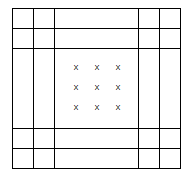
\includegraphics[width=5cm]{figs/7/NSEW_points}
    \caption{NSEW Approach}
    \label{fig:NSEW}
\end{figure}

A method, nicknamed “North, South, East, West” (NSEW) within the project, proposes to shift the 192 pixel focus 32 pixels in each direction to ensure full coverage of the image (as shown in figure \ref{fig:NSEW}). This produces 9 points of focus around the centre of the image, producing 9 attribute vectors per image. The result of this is that every pixel in a tile is covered, with an extra 93\% contextual data gathered from the overlap. This means that every classification decision is made using more information about its surroundings, improving the accuracy. A comparison of the two methods can be observed in figure \ref{fig:NSEW_cover}.


\begin{figure}[H]
    \centering
    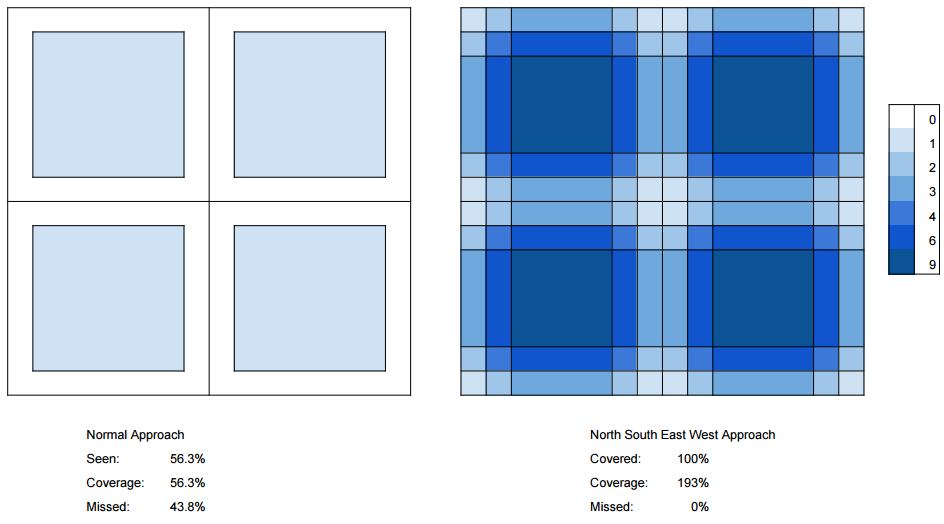
\includegraphics[width=12cm]{figs/7/NSEW}
    \caption{Coverage of NSEW Approach}
    \label{fig:NSEW_cover}
\end{figure}

\section{Implementation}

The core of the modules implementation uses Wilson’s code as a black box. However, to achieve the design, a control or logic layer needed to be included, which required subtle adaptations to the service. These changes will be discussed by the order in which they are used in the flow of the entire system. 

When testing the system, a key bottleneck was downloading the images. This would take considerably longer than processing. Therefore to compensate for this, a new endpoint was introduced ``\textless{}olivia\textgreater{}/download”, which simply accepts a dictionary of image URLs and their tile\_id. Tiles are identified by: \textless{}map\_number\textgreater{}\_\textless{}x\_pos\textgreater{}\_\textless{}y\_pos\textgreater{}. This enabled the service to convert the image on demand rather than waiting for the image to download and convert. This does not reduce the time for the entire process, however through observations of user interactions it was found that the user will not request conversions for considerable time. This time is utilised by downloading the images, as this will occur when they ‘discover’ features later.

The next most expensive operation in the system is the attribute extraction. An observation about this is that no matter how many times you convert an image, the vector returned is always the same, because the DNN  never changes. Therefore once an image is converted, the result can be stored to reduce the best case and average time complexity of conversions to 1, significantly reducing the overall time for a full ‘discover’ sweep.

The first iteration of the service offered the standard convert and the NSEW convert. Both would perform as expected, where the standard convert would perform one conversion per image and NSEW would perform 9 per image. However it was found that the even when a standard convert was requested, the NSEW convert would be requested soon after. Hence in iteration 2, the standard convert would perform the NSEW convert and simply return the middle attribute vector. This reduced the overall computations during the ‘discover’ sweep (that uses NSEW convert). Additionally, since standard converts were often less than 14 images (and 14x9=126 conversions), this would not increase the processing time for standard converts, since 128 conversions can be performed concurrently, explained below. This way the service can extract more data in the same amount of time. 

As the GPU was considered the optimal method for processing extractions, batching had to be managed. Through incremental testing, it was found that 128 concurrent conversions was the perfect balance of stability and performance. This is then complicated by the NSEW approach, as this increases the number of conversion $n$ to $9n$. Ensuring that all nine attributes vectors of an image succeed or fail together is essential to prevent corruption of results. Therefore, a maximum of 14 images can be processed in a single batch, since each image is processed 9 times under NSEW conversions, resulting in 126 conversions with 2 redundantly unused slots.

\section{Testing}
As the system’s most critical sub-module was Wilson’s DNN, this was the first test. To ensure it was behaving correctly, a test image with a known result was passed through to ensure that the expected results match the actual results, on both the last and fourth from the last layer. These unit tests would imply that the DNN has remained unchanged and the modules using it are uncorrupted.

As mentioned, GPU processing was somewhat unreliable with functioning code. To ensure the code was in an optimal state, the batching was unit tested as well as system tested. Other system tests included the NSEW approach, which used test images with coloured 32x32 pixel areas, moved around the image to ensure each of the 9 sections attributes changed only when the coloured area was in their section(see figure \ref{NSEW_test_image} for an example). It was also hand tested to check that a pure white image would provide the same results as sections that couldn’t see the coloured area. There was also a system check script created to run manually to ensure that the GPU processing was configured correctly.

\begin{figure}[H]
    \centering
    
\includegraphics[width=5cm]{figs/7/NSEW_test_img}
    \caption{One of the images used to test NSEW Conversions. The red 32 by 32 pixel squares should only change the results when the focus is shifted to the corners}
    \label{fig:NSEW_test_image}
\end{figure}


\section{Limitations} \label{section:olivia:limits}
The GPU in the machine running Olivia was a Nvidia GTX Titan X with 3072 cuda cores and 12 GB of dedicated RAM. In theory, Olivia should be able to process at least 256 images concurrently, but the amount of RAM proved to be the limiting factor in this instance due to the size of all the images. Therefore, 128 were processed concurrently, halving speed of the attribute extraction.

The minimum tile size is 192 by 192 pixels, which covers quite a large area when using OS’s images. This prevents it from extract attributes about a single feature, since each tile often contains a number of features. For example the data extracted would be correspond to several houses, rather than a single house. 

\section{Evaluation}
This microservice matches the specification; it accepts a tile image and converts it into a collection of attributes. Based on the results seen in chapter \ref{chapter:classifier}, Olivia produces useful attributes. The use of Wilson’s DNN is an evident success. 

Through the discussed techniques, the service has been optimized to reduce the average time required for the full ‘discover’ sweep of the feature finder. These methods, without reducing the time complexity of the service, manipulate the subtleties of usage to pro-actively perform computations when not in demand, and to pause these computations to provide their results when in demand. 

\section{Further Work}
The current NSEW approach results in 9 computations rather than 1. This could be reduced to 5 by only requesting the North East, North West; South East, South West and centre attribute vectors to be produced. This would still cover every pixel of an image, and reduce the computation by roughly half, at the cost of with less accuracy. Experiments could be made to test both extraction methods and determine over an expansive dataset if the tradeoff of reduced accuracy for faster computation time is viable.

A more dramatic improvement would be to entirely retrain the DNN on smaller images. This would allow a more precise feature extraction to occur, combatting the issues mentioned in the limitation section previously (paragraph 2, section \ref{section:olivia:limit§s}). With this there might be less attributes, however the precision gained (through smaller images) would outbalance the negatives.